\documentclass{standalone}

% \input{common.tex}
\usepackage{tikz}
\usetikzlibrary{calc,intersections,through,backgrounds}
\tikzset{
  cut/.style={draw=red,line width=0.1mm},
  marker/.style={draw=green,line width=0.1mm},
  ignore/.style={draw=blue,line width=0.1mm},
}

\begin{document}
\noindent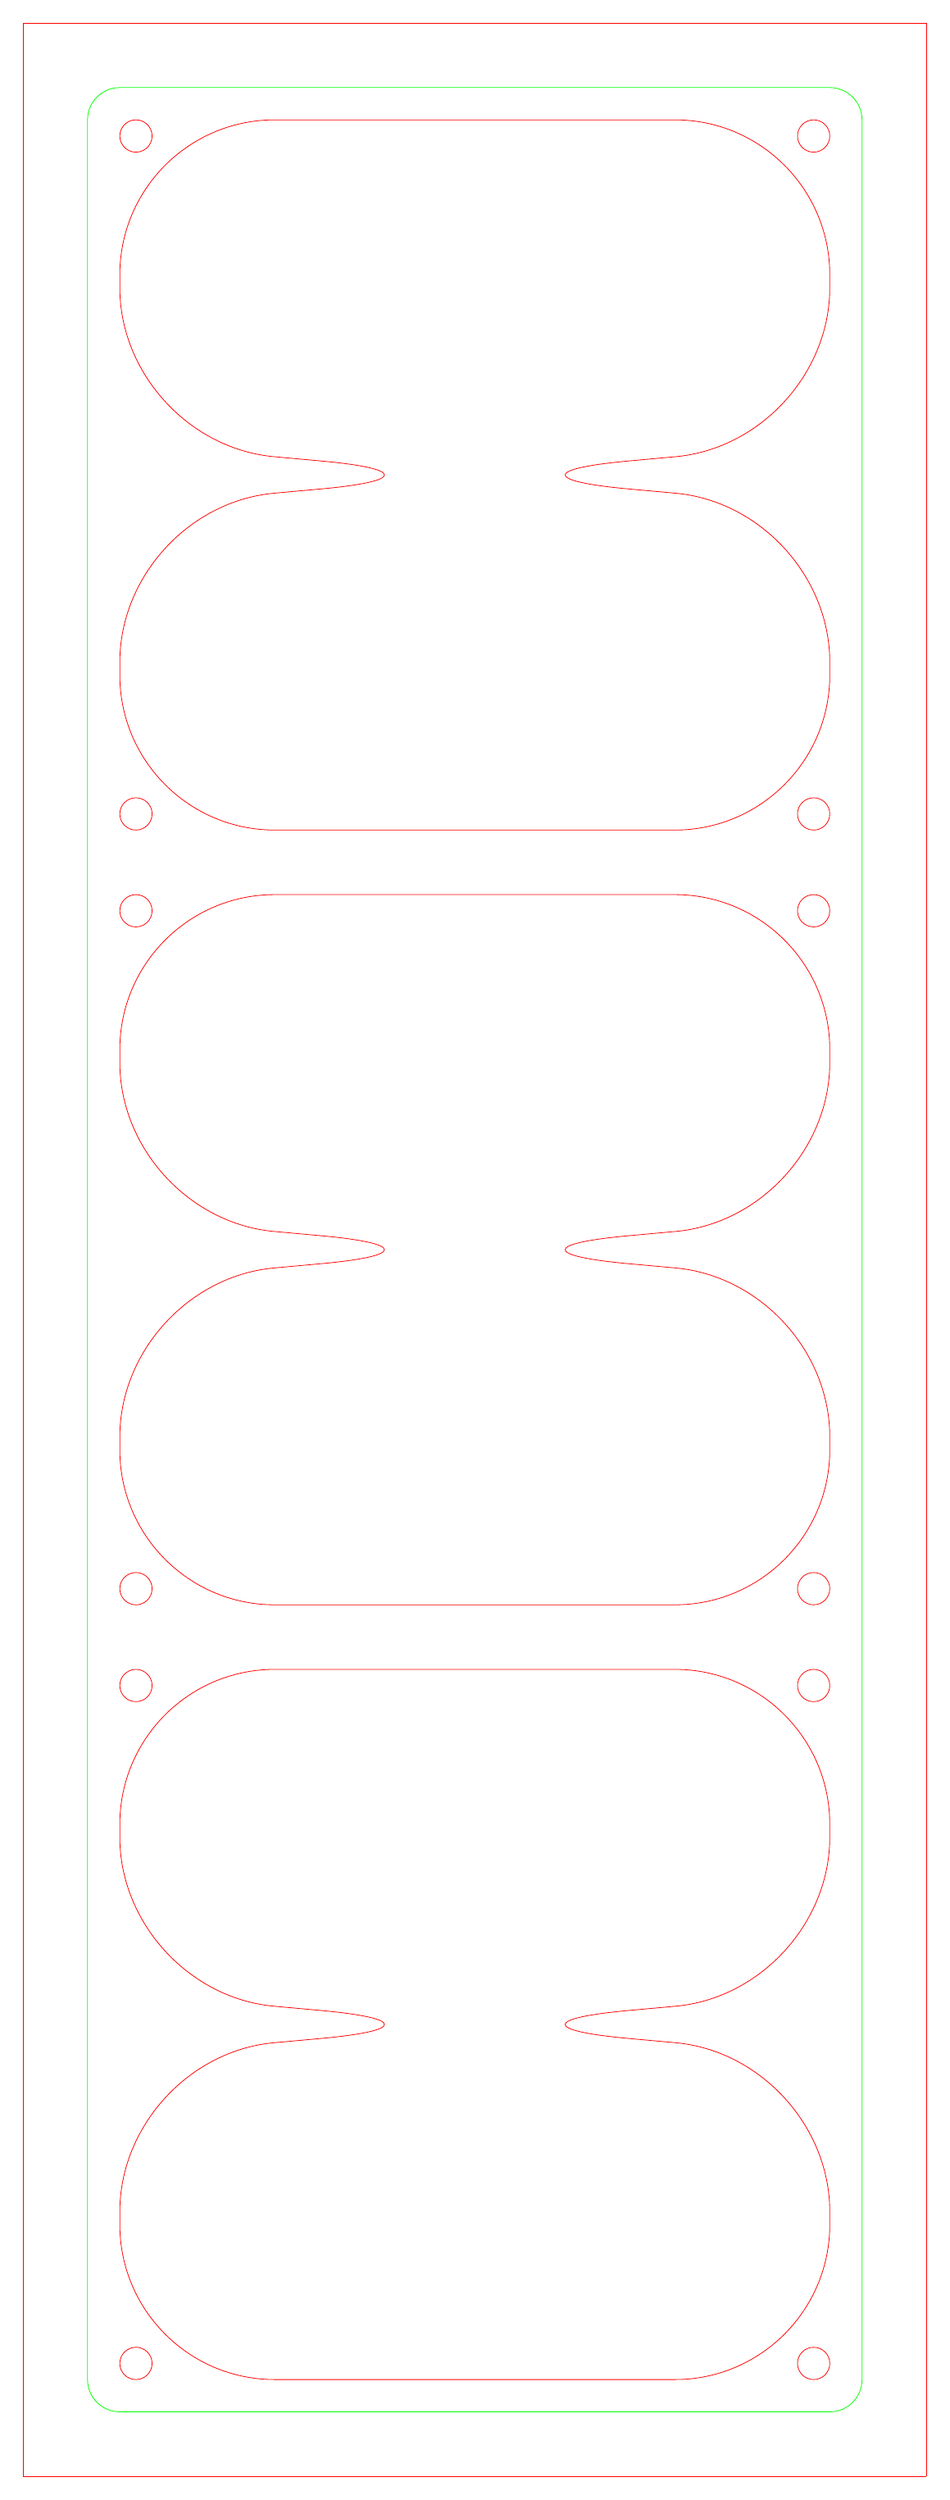
\begin{tikzpicture}[node distance=1cm]
  \foreach \width/\gluewidth/\extramargin/\nfans in {120mm/10mm/10mm/3} {
    \foreach \height in {\nfans * \width} {
      % \path let in node[rectangle,draw=black,line width=0.1mm,minimum height = \height, minimum width=\width] (outline) at (\width / 2, -\height / 2) {};
      \coordinate (se) at (\width + 2 * \extramargin, -\height - 2 * \extramargin);
      \coordinate (sw) at (0, -\height - 2 * \extramargin);
      \coordinate (nw) at (0, 0);
      \coordinate (ne) at (\width + 2 * \extramargin, 0);
      \path let \p1=(sw), \p2=(se), \p3=(nw) in coordinate (dimensions) at (\x2 - \x1, \y3 - \y1);

      \draw[cut] (ne) -- (nw);
      \draw[cut] (nw) -- (sw);
      \draw[cut] (sw) -- (se);
      \draw[cut] (se) -- (ne);

      \coordinate (fan_se) at (\extramargin + \width, -\height - \extramargin);
      \coordinate (fan_sw) at (\extramargin, -\height - \extramargin);
      \coordinate (fan_nw) at (\extramargin, -\extramargin);
      \coordinate (fan_ne) at (\extramargin + \width, -\extramargin);

      \draw[marker,rounded corners = 5mm] (fan_ne) -- (fan_nw) -- (fan_sw) -- (fan_se) -- cycle;

      \foreach \fanindex in {0, 1, 2} {
        \path let \p1=(fan_sw) in coordinate (fancenter) at (\x1 + \width / 2, \y1 + \fanindex * \width + \width / 2);
        %\draw[cut] (fancenter) circle (0.55 * \width); % TODO!

        \path let \p1=(fancenter) in coordinate (fan_inner_ne) at (\x1 + \width / 2 - \gluewidth / 2, \y1 + \width / 2 - \gluewidth / 2);
        \path let \p1=(fancenter) in coordinate (fan_inner_nne) at (\x1 + \gluewidth / 2, \y1 + \width / 2 - \gluewidth / 2);
        \path let \p1=(fancenter) in coordinate (fan_inner_nnw) at (\x1 - \gluewidth / 2, \y1 + \width / 2 - \gluewidth / 2);
        \path let \p1=(fancenter) in coordinate (fan_inner_nw) at (\x1 - \width / 2 + \gluewidth / 2, \y1 + \width / 2 - \gluewidth / 2);
        \path let \p1=(fancenter) in coordinate (fan_inner_wnw) at (\x1 - \width / 2 + \gluewidth / 2, \y1 + \gluewidth / 2);
        \path let \p1=(fancenter) in coordinate (fan_inner_wsw) at (\x1 - \width / 2 + \gluewidth / 2, \y1 - \gluewidth / 2);
        \path let \p1=(fancenter) in coordinate (fan_inner_sw) at (\x1 - \width / 2 + \gluewidth / 2, \y1 - \width / 2 + \gluewidth / 2);
        \path let \p1=(fancenter) in coordinate (fan_inner_ssw) at (\x1 - \gluewidth / 2, \y1 - \width / 2 + \gluewidth / 2);
        \path let \p1=(fancenter) in coordinate (fan_inner_sse) at (\x1 + \gluewidth / 2, \y1 - \width / 2 + \gluewidth / 2);
        \path let \p1=(fancenter) in coordinate (fan_inner_se) at (\x1 + \width / 2 - \gluewidth / 2, \y1 - \width / 2 + \gluewidth / 2);
        \path let \p1=(fancenter) in coordinate (fan_inner_ese) at (\x1 + \width / 2 - \gluewidth / 2, \y1 - \gluewidth / 2);
        \path let \p1=(fancenter) in coordinate (fan_inner_ene) at (\x1 + \width / 2 - \gluewidth / 2, \y1 + \gluewidth / 2);

        % \draw[cut,rounded corners = \width / 4] (fan_inner_ne) -- (fan_inner_nw) -- (fan_inner_sw) -- (fan_inner_se) -- cycle;
        \draw[cut,rounded corners = \width / 5] (fan_inner_ne) -- %(fan_inner_nne) -- (fancenter) -- (fan_inner_nnw) --
        (fan_inner_nw) -- (fan_inner_wnw) -- (fancenter) -- (fan_inner_wsw) --
        (fan_inner_sw) -- %(fan_inner_ssw) -- (fancenter) -- (fan_inner_sse) --
        (fan_inner_se) -- (fan_inner_ese) -- (fancenter) -- (fan_inner_ene) --
        cycle;
        
        \foreach \holecenterdistance in {\width * 0.5 - 7.5mm} { % TODO: Adjust/Test for non-120mm fans
          \foreach \xholeindex in {-1, 1} {
            \foreach \yholeindex in {-1, 1} {
              \path let \p1=(fan_sw), \p2=(\holecenterdistance, \holecenterdistance) in coordinate (holeposition) at (\x1 + \width / 2 + \x2 * \xholeindex, \y1 + \width * \fanindex + \width / 2 + \x2 * \yholeindex);
              \draw[cut] (holeposition) circle (2.5mm); % TODO!
            }
          }
        }
      }
    }
  }
\end{tikzpicture}
\end{document}